% (c) 2014 Claudio.carboncinii - claudio.carboncini@gmail.com
% (c) 2014 Dimitrios Vrettos - d.vrettos@gmail.com
\chapter{Numeri reali}
\section{Dai numeri naturali ai numeri irrazionali}
Nel volume Algebra 1 abbiamo presentato i diversi insiemi numerici. Li riprendiamo brevemente per poi approfondire i numeri reali e le loro proprietà.

L'insieme dei \emph{numeri naturali} racchiude i numeri che utilizziamo per contare; si indica nel seguente modo:
\[\insN=\{0,1,2,3,4,5,6,7,8,9,10,11,\ldots\}\]

Su questi numeri sono definite le seguenti operazioni:
\begin{itemize*}
 \item \emph{addizione}: $n+m$ è il numero che si ottiene partendo da $n$ e continuando a contare per altre $m$ unità;
 \item \emph{sottrazione}: $n-m$ è il numero, se esiste ed è unico, che addizionato a $m$ dà come risultato $n$;
 \item \emph{moltiplicazione}: $n \cdot m$ è il numero che si ottiene sommando $n$ volte $m$, o meglio sommando $n$ addendi tutti uguali a $m$;
 \item \emph{divisione}: $n:m$ è il numero, se esiste ed è unico, che moltiplicato per $m$ dà come risultato $n$;
 \item \emph{potenza}: $n^{m}$ è il numero che si ottiene moltiplicando $m$ fattori tutti uguali a $n$ con $m \ge 2$, ponendo $n^{1}=n$ e $n^{0}=1$;
 \item \emph{radice}: $\sqrt[{n}]{m}$ con $n\ge 2$ è il numero, se esiste ed è unico, che elevato a $n$ dà come risultato $m$.
\end{itemize*}

L'addizione, la moltiplicazione e la potenza sono definite su tutto l'insieme dei numeri naturali, cioè dati due numeri naturali qualsiasi, $n$ ed $m$, la somma $n+m$ e il loro prodotto $n \cdot m$ è sempre un numero naturale; la potenza $n^{m}$, escluso il caso $0^{0}$, è un numero naturale. Non sempre, invece, è possibile calcolare la differenza $n-m$, il quoziente $n:m$ o la radice $\sqrt[{n}]{m}$.

Tuttavia, dal punto di vista pratico-applicativo molto spesso si incontrano situazioni nelle quali occorre eseguire sempre operazioni. Iniziamo dall'operazione di sottrazione. Sappiamo che in tante situazioni di natura economica, ma non solo, deve essere possibile sottrarre un numero da uno più piccolo. Deve essere possibile, per esempio, comprare un'auto che costa 12.000 euro anche quando in banca possediamo solo 10.000 euro. Deve quindi essere possibile eseguire una sottrazione del tipo $10.000-12.000$. Il risultato di questa operazione non va poi confuso con il risultato di $12.000-10.000$. Nel secondo caso, infatti, significa che sul nostro conto corrente abbiamo 12.000 euro e dobbiamo spenderne 10.000, ci rimangono quindi 2.000 euro. Nel primo caso invece, possediamo 10.000 euro e dobbiamo pagare
12.000 euro ci rimane un debito di 2.000 euro. Per distinguere i due tipi di numeri i matematici mettono davanti al numero il segno $+$ o il segno $-$. Si genera così l'insieme dei \emph{numeri relativi}.
\[\insZ=\{\ldots,-3,-2,-1,0,+1,+2,+3,\ldots\}\]
Su questi numeri l'operazione di sottrazione è ovunque definita, in altre parole è possibile eseguire tutte le sottrazioni.

Non è invece possibile eseguire sempre le divisioni. Oltre hai casi $n:0$ e $0:0$, non è possibile, con i numeri interi, eseguire la divisione $3:4$. Esistono però tante situazioni reali in cui una divisione di questo tipo deve poter essere eseguita. Per esempio è possibile dividere in parti uguali 3 uova in 4 persone, basta fare una frittata in una padella tonda e dividere la frittata in quattro parti uguali, a ciascuna toccano $\frac{3}{4}$ di uovo. Deve
essere possibile dividere in parti uguali 3 euro tra 4 persone. Dopo aver notato che a nessuno tocca 1 euro intero, si procede a cambiare le monete da 1 euro in monete da 1 decimo di euro, si cambiano quindi i 3 euro con 30 decimi di euro. Dividendo le 30 monete in 4 parti uguali risulta che ciascuno riceve 7 monetine e ne avanzano 2. Per dividere le 2 monete da un decimo si cambiano in monete da un centesimo, ottenendo 20 centesimi di euro. Si dividono allora le 20 monetine in 4 parti uguali, ciascuno avrà 5 centesimi di euro. In tutto a ciascuno toccano 75 centesimi di euro.

Per rappresentare il risultato di queste due operazioni di divisioni abbiamo usato nel primo caso la notazione frazionaria $\frac{3}{4}$ e nel secondo caso la notazione decimale $0,75$. Le due scritture sono perfettamente equivalenti.

Per risolvere tutti i problemi di divisione i matematici hanno costruito l'insieme dei \emph{ numeri razionali} che indichiamo nel seguente modo:
\[
\insQ=\left\{\frac{n}{m} \mid n\in \insZ,m\in \insN,m\neq
0\right\}=\left\{0,+1,-1,\frac{1}{2},-\frac{1}{2},+\frac{2}{3,}-\frac{1}{5},-\frac{11}{17},\frac{129}{1725}...\right\}
\]

Con questi numeri è possibile sempre eseguire l'addizione, la sottrazione, la moltiplicazione, la divisione (ad eccezione della divisione per 0), la potenza. Non sempre, invece, è possibile eseguire l'estrazione di radice. Per esempio, hai già conosciuto il numero $\sqrt{2}$, cioè il numero che elevato al quadrato dà 2; esso non è un numero razionale, cioè non può essere scritto né sotto forma di frazione né sotto forma di numero decimale finito o periodico. I numeri di questo tipo si dicono \emph{numeri irrazionali}.

Abbiamo già affrontato questo problema nel volume di Algebra 1; per comodità del lettore riportiamo il ragionamento.

Fissiamo sulla retta orientata~$r$ l'unità di misura e disegniamo il quadrato di lato~1. Ci proponiamo di calcolare
la misura della sua diagonale~$OB$.

\begin{center}
 % (c) 2013 Claudio Carboncini - claudio.carboncini@gmail.com
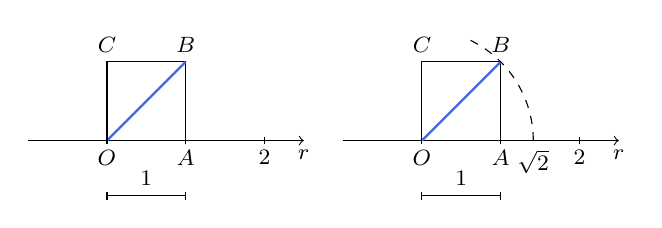
\begin{tikzpicture}[x=10mm, y=10mm, font=\footnotesize]
  \draw [->] (0,0) -- (3.5,0) node [below] () {$r$};
  \draw (1,0) rectangle (2,1);
  \draw[RoyalBlue, thick] (1,0) -- (2,1);

  \coordinate[label=below:$O$] (O) at (1,0);
  \coordinate[label=below:$A$] (A) at (2,0);
  \coordinate[label=above:$C$] (C) at (1,1);
  \coordinate[label=above:$B$] (B) at (2,1);

  \foreach \x in {1,...,3}{
    \draw (\x,-0.5mm) -- (\x,0.5mm);
  }
  \node[below] at (3,0) {2};
  
  \begin{scope}[yshift=-7mm]
    \draw (1,0) -- (2,0);
    \draw (1,-0.5mm) -- (1,0.5mm);
    \draw (2,-0.5mm) -- (2,0.5mm);
    \node[above] at (1.5,0) {1};
  \end{scope}
  
  \begin{scope}[xshift=40mm]
    \draw [->] (0,0) -- (3.5,0) node [below] () {$r$};
    \draw (1,0) rectangle (2,1);
    \draw[RoyalBlue, thick] (1,0) -- (2,1);

    \coordinate[label=below:$O$] (O) at (1,0);
    \coordinate[label=below:$A$] (A) at (2,0);
    \coordinate[label=above:$C$] (C) at (1,1);
    \coordinate[label=above:$B$] (B) at (2,1);
    \coordinate[label=below:$\sqrt{2}$] (K) at (2.414,0);

    \draw[dashed] (2.414,0) arc [start angle=0, end angle=65,radius=1.414cm];

    \foreach \x in {1,...,3}{
      \draw (\x,-0.5mm) -- (\x,0.5mm);
    }
    \node[below] at (3,0) {2};
  
    \begin{scope}[yshift=-7mm]
      \draw (1,0) -- (2,0);
      \draw (1,-0.5mm) -- (1,0.5mm);
      \draw (2,-0.5mm) -- (2,0.5mm);
      \node[above] at (1.5,0) {1};
    \end{scope}

  \end{scope}
\end{tikzpicture}
\end{center}

Il triangolo~$OAB$ è retto in~$A$, quindi per il teorema di
Pitagora~$\overline{OB}^{2}=\overline{OA}^{2}+\overline{AB}^{2}$.
Sostituiamo le misure:~$\overline{OB}^{2}=1^2+1^2=2$. Per ottenere~$\overline{OB}$
dobbiamo estrarre la radice quadrata e quindi~$\overline{OB}=\sqrt{2}$.

Sappiamo che `estrarre la radice quadrata' di un numero significa trovare quel numero
che elevato al quadrato dà~2. Questo numero deve esistere, nel senso
che esiste un punto sulla retta~$r$ che lo rappresenta, per costruirlo graficamente si può tracciare l'arco di
circonferenza di centro~$O$ e raggio~$OB$ determinando su $r$ il punto~$K$ estremo del segmento con~$OK = OB$.

Dalla posizione del punto~$K$ possiamo dire che~$1<\sqrt{2}<2$. Il
valore cercato evidentemente non è un numero intero. Può essere un
numero decimale finito? Compiliamo una tabella che contenga nella prima
riga i numeri con una sola cifra decimale compresi tra~1 e~2 e nella
seconda riga i rispettivi quadrati:

\begin{center}
\begin{tabular}{ccccccc}
\toprule
$x$ & 1,1 & 1,2 & 1,3 & 1,4 & 1,5 & 1,6\\
$x^{2}$ & 1,21 & 1,44 & 1,69 & 1,96 & 2,25 & 2,89\\
\bottomrule
\end{tabular}
\end{center}

Osserviamo che il numero~2 è compreso tra~$1,4^{2}$ e~$1,5^{2}$,
di conseguenza~$1,4<\sqrt{2}<1,5$, ma ancora
non possiamo precisare il suo valore, anche se abbiamo ristretto
l'intervallo in cui si trova il punto~$K$. Diciamo che~1,4 è un valore approssimato per
difetto di~$\sqrt{2}$ mentre~1,5
è un valore approssimato per eccesso; scrivendo~$\sqrt{2}=1,4$
oppure~$\sqrt{2}=1,5$ commettiamo un errore minore di~1/10.

Per migliorare l'approssimazione e tentare di ottenere~$\sqrt{2}$
come numero razionale costruiamo la tabella dei numeri
decimali con due cifre compresi tra~1,4 e~1,5:

\begin{center}
\begin{tabular}{ccccc}
\toprule
$x$ &1,41 &1,42 &1,43 &1,44\\
$x^{2}$ & 1,9881 & 2,0164 & 2,0049 & 2,0776\\
\bottomrule
\end{tabular}
\end{center}

Ora possiamo dire che~1,41 è un valore approssimato per difetto di~$\sqrt{2}$ mentre~1,42 è un valore approssimato
per eccesso, con un errore dell'ordine di~1/100. Abbiamo quindi migliorato
l'approssimazione e di conseguenza abbiamo ristretto l'intervallo in cui cade il punto~$K$, ma ancora non
abbiamo trovato un numero razionale che sia uguale a~$\sqrt{2}$.

Continuando con lo stesso procedimento costruiamo due classi di numeri razionali che approssimano una per difetto e
una per eccesso il numero cercato, restringendo ogni volta l'ampiezza dell'intervallo in cui cade il punto~$K$.
Il procedimento continua all'infinito e le cifre decimali che troviamo non si ripetono periodicamente.

\begin{center}
 \begin{tabular}{lcll}
\toprule
Valore per difetto & Numero &Valore per eccesso & Ordine dell'errore\\
\midrule
1	& $\sqrt{2}$ 	& 2 	&1\\
1,4	& $\sqrt{2}$	&1,5 	& $10^{-1}$\\
1,41	& $\sqrt{2}$	& 1,42	& $10^{-2}$\\
1,414	& $\sqrt{2}$	&1,415	&$10^{-3}$\\
1,4142	& $\sqrt{2}$	& 1,4143&$10^{-4}$\\
\ldots	& $\sqrt{2}$	&\ldots	&\ldots\\
\bottomrule
\end{tabular}
\end{center}

Per arrivare a concludere che~$\sqrt{2}$ non è un numero razionale,
possiamo ragionare nel seguente modo. Supponiamo per assurdo che~$\sqrt{2}$
sia un numero razionale e precisamente $\sqrt{2}=\frac{a}{b}$ con~$a$ e~$b$ primi tra loro. Se si eleva al quadrato $\sqrt{2}$ si ottiene $2=\frac{a^{2}}{b^{2}}$.

Elevare un numero al quadrato significa elevare al quadrato le
singole potenze dei fattori primi in cui questo si scompone. I fattori
primi di~$a^{2}$ e di~$b^{2}$ sono gli stessi di~$a$ e di~$b$ con
gli esponenti raddoppiati, anche~$a^{2}$ e~$b^{2}$
sono primi tra di loro e~$a^{2}$ non può essere il doppio di~$b^{2}$.
Quindi~$2\ne\frac{a^{2}}{b^{2}}$ e~$\sqrt{2}\ne\frac{a}{b}$.

Oltre a $\sqrt{2}$ vi sono altri infiniti numeri che non possono essere scritti come frazione. Per esempio, tutte le radici quadrate di numeri naturali che non sono quadrati perfetti e tutte le radici quadrate di frazioni che non sono il quadrato di alcuna frazione. Ma anche le radici cubiche del tipo $\sqrt[{3}]{2}$, $\sqrt[{5}]{7}$, {\dots} Un altro famoso numero irrazionale che si incontra nelle misure geometriche è il numero $\pi$, che corrisponde alla
misura della circonferenza di diametro $1$.

Questi numeri sono detti \emph{numeri irrazionali} e insieme ad altri, come $\pi$ ed altri ancora che conoscerete in seguito, costituiscono l'insieme $\insJ$ dei numeri irrazionali.

L'unione degli insiemi $\insQ$ e $\insJ$ è l'insieme $\insR$ dei numeri reali.

\vspazio\ovalbox{\risolvii \ref{ese:1.1}, \ref{ese:1.2}}

\section{I numeri reali}
In base a quanto abbiamo detto prima, essendo $\insR=\insQ \cup \insJ$, i numeri reali sono tutti quei numeri che si possono scrivere in forma decimale con un numero finito o infinito di cifre, non necessariamente periodiche.
Per esempio, la frazione $\dfrac{17}{16}$ è uguale al numero decimale finito~1,0625.
La frazione $\dfrac{16}{17}$ è uguale al numero decimale periodico $0,\overline{9411764705882352}$.

Il numero $\pi$ è invece un numero decimale a infinite cifre non periodico. Riportiamo alcune cifre:
$\pi $ = 3, 141 592 653 589 793 238 462 643 383 279 502 884 197 169 399 375 105 820 974 944 592 307 816 406 286
208 998 628 034 825 342 117 067 982 148 086 513 282 306 647 093 844 609 550 582 231 725 359 408 128 481 117 450 284 102
701 938 521 105 559 644 622 948 954 930 381 964 428 810 975 665 933 446 128 475 648 233 786 783 165 271 201 909 145 648
566 923 460 348 610 454 326 648 213 393 607 260 \ldots Nonostante i numeri irrazionali siano stati scoperti dallo stesso Pitagora o dai suoi allievi nel $IV$~secolo~$\aC$, solo nel $XIX$~secolo Augustin-Louis Cauchy e Richard Dedekind sono giunti a una formulazione rigorosa di numeri reali.

In effetti, assumere che i numeri reali sono tutti quelli che si possono scrivere in forma decimale finita o infinita, del tipo $r=n+0,abcd\ldots$, dove $r$ è il numero reale, $n$ è la parte intera e $0,abcd\ldots$ è la parte decimale, comporta dei problemi. Per esempio, i numeri interi hanno una doppia rappresentazione: $1=0,99999999\ldots$ come i numeri decimali finiti: $1,225=1,22499999999\ldots$ Occorre quindi almeno escludere i numeri decimali con il~9 periodico. Oltre questo problema rimane la difficoltà di eseguire le operazioni tra numeri decimali illimitati. Gli algoritmi per addizionare, sottrarre e moltiplicare due numeri richiedono di cominciare dall'ultima cifra, cosa che non è possibile per i numeri decimali che non finiscono mai. Altro problema non semplice da gestire è il fatto che una definizione di
questo tipo è strettamente legata al sistema di numerazione a base 10 che noi utilizziamo.

Già nel volume Algebra 1, nel paragrafo sulle relazioni di equivalenza, abbiamo visto come i matematici hanno potuto costruire l'insieme $\insZ$ degli interi relativi a partire dall'insieme di coppie ordinate di $\insN \times \insN$ e l'insieme $\insQ$ dei razionali relativi a partire dall'insieme di coppie ordinate di $\insZ \times \insZ_{0}$.

La questione a questo punto è: possiamo costruire l'insieme dei numeri reali a partire dall'insieme dei numeri razionali $\insQ$? Per rappresentare il numero $\sqrt{2}$ abbiamo costruito un insieme, che abbiamo indicato con $A$, di numeri razionali il cui quadrato è minore di $2$ e un insieme, che abbiamo indicato con $B$, di numeri razionali il cui quadrato è maggiore di $2$. Sembra allora che il numero $\sqrt{2}$ spezzi l'insieme dei numeri razionali $\insQ$ in due parti: quella dei numeri razionali $a$ tali che $a^{2}<2$ e quella dei numeri razionali $b$ tali che $b^{2}>2$. La coppia di insiemi $(A,B)$ caratterizza il numero $\sqrt{2}$, possiamo anzi identificare $\sqrt{2}$ con la coppia $(A,B)$.

È proprio questa l'idea alla base del ragionamento del matematico tedesco Dedekind~(1831-1916). Dedekind chiama \emph{sezione}, o \emph{partizione} di $\insQ$, una coppia di sottoinsiemi non vuoti $A$ e $B$ che devono soddisfare le condizioni: $A \cap B=\emptyset$; $A \cup B=\insQ$; $\forall a \in A, \forall b \in B, a<b$.

\begin{exrig}
 \begin{esempio}
 Sezioni
 \begin{itemize}
 \item Consideriamo i due insiemi $A$ e $B$ così definiti: $A=\left\{x\in \insQ |\, x<3\right\}$,
$B=\left\{x\in \insQ |\, x \ge 3\right\}$. Essi definiscono una sezione di $\insQ$, infatti
$A \cap B=\emptyset$; $A \cup B=\insQ$ e ogni elemento di A è minore di ogni elemento di B; inoltre possiamo osservare che $A$ non ammette massimo, non essendoci in esso un numero che sia maggiore di tutti gli altri, mentre $B$ ammette il minimo che è 3;
 \item siano $A=\left\{x\in \insQ |\, x<-1\right\}$, $B=\left\{x \in \insQ |\, x>0\right\}$ la coppia $(A,B)$ non è una sezione di $\insQ$ perché pur essendo $A\cap B=\emptyset$ non è $A\cup B=\insQ$;
 \item siano $A=\left\{x\in \insQ |\, x \le \frac{2}{7}\right\}$, $B=\left\{x \in Q |\, x \ge \frac{2}{7}\right\}$, anche in questo caso la coppia $(A,B)$ non è una sezione di $\insQ$ poiché $A\cap B=\left\{\frac{2}{7}\right\}$;
 \item costruiamo gli insiemi $A$ e $B$ nel seguente modo: $A$ sia l'unione tra l'insieme dei numeri razionali negativi e tutti i razionali il cui quadrato è minore di 2, in $B$ mettiamo tutti i razionali il cui quadrato è maggiore di 2. $A=\insQ^{-} \cup \left\{x \in \insQ |\, x^{2}<2\right\}$, $B=\left\{x \in \insQ |\, x^{2}>2\right\}$. Si ha $A \cap B=\emptyset$; $A\cup B=\insQ$, inoltre ogni elemento di $A$ è minore di ogni elemento di $B$, dunque $(A,B)$ è una sezione di $\insQ$, ma $A$ non possiede il massimo e $B$ non possiede il minimo, in quanto abbiamo già dimostrato che non esiste un numero razionale che ha $2$ come quadrato. Questa sezione individua un buco nell'insieme $\insQ$.
 \end{itemize}
 \end{esempio}
\end{exrig}

Gli esempi visti ci permettono di affermare che una partizione $(A,B)$ può essere di tre tipi:
\begin{itemize*}
\item $A$ ammette massimo e $B$ non ammette minimo;
\item $A$ non ammette massimo e $B$ ammette minimo;
\item $A$ non ammette massimo e $B$ non ammette minimo.
\end{itemize*}

\begin{definizione}
Si chiama \emph{elemento separatore} di una partizione $(A,B)$ di $\insQ$ il massimo di $A$ o il minimo di $B$, nel caso in cui almeno uno di questi elementi esista.
\end{definizione}

Nel primo esempio, poiché esiste il minimo di $B$, la partizione $(A,B)$ ammette un elemento separatore e identifica il numero razionale $3$.
Nel quarto esempio non esiste un numero razionale che fa da elemento separatore, la sezione $(A,B)$ identifica un numero irrazionale.

\begin{definizione}
L'insieme $\insR$ dei numeri reali è l'insieme di tutte le partizioni di $\insQ$. Chiamiamo
numero razionale le partizioni che ammettono elemento separatore, chiamiamo \emph{numero irrazionale} le sezioni che non ammettono elemento separatore.
\end{definizione}

Ogni numero reale è individuato da due insiemi di numeri razionali: nel primo tutte le approssimazioni per difetto e nell'altro tutte le approssimazioni per eccesso.

Ritornando all'esempio precedente, il numero $\sqrt{2}$ è individuato dalla sezione costituita dagli insiemi $A=\left\{x\in \insQ |\, x<0\right\}$ oppure $x^{2}<2$ e $B=\left\{x\in \insQ |\, x^{2}>2\right\}$.
Nell'insieme $A$ ci sono tutti i numeri razionali negativi oltre quelli che approssimano $\sqrt{2}$ per difetto: \[A=\{1;1,4;1,41;1,414;1,4142;1,414213;\ldots\}.\]
Nell'insieme B ci sono tutti i numeri razionali che approssimano $\sqrt{2}$ per eccesso:
\[B=\{2;1,5;1,42;1,415;1,4143;1,41422;1,414214;\ldots\}.\]

Questa costruzione dell'insieme dei numeri reali $\insR$ a partire dall'insieme dei numeri razionali
$\insQ$ è puramente astratta e formale, non serve al calcolo, vuole solo concludere il cammino intrapreso per costruire tutti gli insiemi numerici a partire dall'insieme dei numeri naturali $\insN$.

Dal punto di vista teorico è possibile definire nell'insieme delle partizioni di $\insQ$, l'ordinamento e le operazioni. Dal punto di vista del calcolo useremo le approssimazioni.

\begin{definizione}
Un insieme $X$ si dice \emph{continuo} se ogni partizione $(X', X'')$ di $X$ ammette uno e un solo elemento separatore, cioè se esiste un elemento $x$ appartenente a $X$ tale che per ogni $x'$ di $X'$ e per ogni $x''$ di $X''$ si ha $x'{\leq}x{\leq}x''$.
\end{definizione}

\begin{teorema}[di Dedekind]
Ogni partizione dell'insieme $\insR$ di numeri reali ammette uno e uno solo elemento separatore.
\end{teorema}

Da questo teorema segue che il numero reale è definito come l'elemento separatore di una sezione $(A,B)$ di numeri reali.

\begin{postulato}[di continuità della retta]
Esiste una corrispondenza biunivoca tra l'insieme dei punti della retta geometrica e l'insieme $\insR$ dei numeri reali.
\end{postulato}

Da questo postulato segue la possibilità di definire sulla retta un sistema di coordinate: ad ogni punto corrisponde un numero reale (la sua ascissa) e viceversa ad ogni numero reale è associato uno e un solo punto sulla retta; analogamente si ha nel piano dove il sistema di assi cartesiano permette di realizzare una corrispondenza biunivoca tra coppie di numeri reali (ascissa e ordinata del punto) e un punto del piano geometrico. Vedremo in seguito che la possibilità di associare numeri e punti si estende anche allo spazio geometrico.

\subsection{Confronto fra numeri reali}
Per confrontare due numeri reali, osserviamo prima di tutto i segni. Se i segni dei numeri sono
discordi, il numero negativo è minore del numero positivo. Se i segni dei numeri sono concordi si valuta la parte intera del numero: se sono positivi è più grande quello che ha la parte intera maggiore, viceversa se sono negativi è più grande quello che ha la parte intera minore. A parità di parte intera bisogna confrontare la parte decimale partendo dalle cifre più a sinistra finché non si trova la prima cifra decimale diversa: se i numeri sono positivi è maggiore quello che ha la cifra maggiore; se sono negativi è maggiore quello che ha la cifra minore.

\begin{exrig}
 \begin{esempio}
 Confrontare i seguenti numeri reali
 \begin{itemize}
 \item $\sqrt{2}<\sqrt{3}$ per verificarlo ci si può aiutare con la calcolatrice per calcolare le prime cifre decimali dei due numeri $\sqrt{2}=1,4142\ldots$, $\sqrt{3}=1,7320\ldots$; oppure ci si arriva osservando che il numero che elevato al quadrato dà 2 deve essere minore del numero che elevato al quadrato dà 3;
 \item $\sqrt{99}<10$ per verificarlo è sufficiente osservare che $\sqrt{100}=10$.
 \end{itemize}
 \end{esempio}
\end{exrig}
\ovalbox{\risolvii \ref{ese:1.3}, \ref{ese:1.4}, \ref{ese:1.5}, \ref{ese:1.6}, \ref{ese:1.7}}\vspazio

\section{Richiami sul valore assoluto}

Si definisce \emph{valore assoluto} di un numero reale $a$, indicato con $\valass{a}$, il numero stesso se $a$ è positivo o nullo, il suo opposto se $a$ è negativo.

\[
|a|=\left\{\begin{array}{l}
a\text{, se }a\ge~0\\
-a\text{, se }a<0\end{array}.\right.
\]

Il numero $a$ si dice argomento del valore assoluto.
\begin{multicols}{3}
$\valass{-3}=3$;\\$\valass{+5}=5$;\\$\valass{0}=0$.
\end{multicols}
\subsection{Proprietà del valore assoluto}
$\valass{x+y}\le \valass{x}+\valass{y}$: il valore assoluto della somma di due numeri è minore o uguale della somma dei valori assoluti dei due numeri. Si ha l'uguaglianza solo quando i due numeri reali hanno lo stesso segno, oppure quando almeno uno dei due numeri è nullo.

$\valass{x-y}\le \valass{x}+\valass{y}$: il valore assoluto della differenza di due numeri è minore o uguale della somma dei valori assoluti dei due numeri.

$\valass{x\cdot y}=\valass{x}\cdot \valass{y}$: il valore assoluto del prodotto di due numeri
è uguale al prodotto dei valori assoluti dei due numeri.

$\left |{\dfrac{x}{y}}\right|=\dfrac{\valass{x}}{\valass{y}}$: il valore assoluto del rapporto di due
numeri è uguale al rapporto dei valori assoluti dei due numeri.

In generale, se l'argomento del valore assoluto è una funzione $f(x)$ si ha:
\[
\valass{f(x)}=\left\{\begin{array}{l}
f(x) \text{, se }f(x)\ge~0\\
-f(x)\text{, se }f(x)<0\end{array}.\right.
\]
\begin{exrig}
 \begin{esempio}
 Valore assoluto di numeri reali
 \begin{itemize}
 \item $\valass{5+3}=\valass{5}+\valass{3}$ in entrambi i casi si ottiene $8$;
 \item $\valass{5+(-3)}=2$ mentre $\valass{5}+\valass{-3}=8$, pertanto $\valass{5+(-3)}<\valass{5}+\valass{-3}$.
 \end{itemize}
 \end{esempio}
\end{exrig}

Nelle espressioni contenenti valori assoluti di argomento letterale si deve cercare di eliminare il
valore assoluto.

\begin{exrig}
 \begin{esempio}
 Valore assoluto di argomento letterale
 \begin{itemize}
 \item $\left|{x^{2}}\right|=x^{2}$ infatti $x^{2}$ è una quantità sempre non negativa;
 \item $\left|{a^{2}+1}\right|=a^{2}+1$ infatti $a^{2}$ è sempre positivo, aumentato di $1$ sarà sempre $>0$;
 \item $\valass{x-1}=\left\{\begin{array}{l}
x-1\text{, se }x\ge~1\\
-x+1\text{, se }x<1\end{array}\right.$ una funzione di questo tipo si dice \emph{definita per casi};
 \item $f(a)=\valass{a+1}-3a+1$ acquista due significati a seconda che l'argomento del valore assoluto sia non negativo o negativo. La sua espressione algebrica è:
\[
f(a)=\valass{a+1}-3a+1=\left\{\begin{array}{l}
a+1-3a+1=-2a+2 \text{, se }a+1\ge~0\Rightarrow a\ge-1\\
-(a+1)-3a+1=-4a \text{, se }a+1<~0\Rightarrow a<-1\end{array}.\right.
\]
 \end{itemize}
 \end{esempio}
\begin{esempio}
 $f(x)=\valass{x-5}+\valass{x+2}$.

 La presenza di due valori assoluti ci obbliga a studiare i casi generati dal segno dei singoli argomenti.
 Pertanto poiché l'argomento del primo valore assoluto è non negativo per $x\ge 5$ e l'argomento del secondo valore assoluto è non negativo
 per $x\ge -2$, possiamo porre la reciproca situazione nel seguente grafico:
\begin{center}
\input{./lbr/chap01/fig002_rad2.pgf}
\end{center}

\begin{enumerate}[label={(\Alph*)}]
 \item $x<-2$: in questo intervallo entrambi gli argomenti sono negativi, pertanto 
\[f(x)=\valass{x-5}+\valass{x+2}=-x+5-x-2=-2x+3.\]
Se $x=-2$ si ha $f(-2)=\valass{-2-5}+0=7$;
 \item $-2<x<5$ il primo argomento è negativo e il secondo è positivo, pertanto 
\[f(x)=\valass{x-5}+\valass{x+2}=-x+5+x+2=7.\]
Se $x=5$ si ha $f(5)=0+\valass{5+2}=7$;
 \item $x>5$ entrambi gli argomenti positivi, pertanto 
\[f(x)=\valass{x-5}+\valass{x+2}=x-5+x+2=2x-3.\]
\end{enumerate}
Possiamo allora sintetizzare in questo modo
\[
\valass{x-5}+\valass{x+2}=\left\{\begin{array}{l}
-2x+3 \text{, se }x<-2\\
7 \text{, se }-2\le x<5\\
2x-3 \text{, se }x\ge 5\end{array}.\right.
\]
\end{esempio}
\end{exrig}
\ovalbox{\risolvii \ref{ese:1.7}, \ref{ese:1.8}, \ref{ese:1.9}, \ref{ese:1.10}, \ref{ese:1.11}}

\newpage

% (c)~2014 Claudio Carboncini - claudio.carboncini@gmail.com
% (c)~2014 Dimitrios Vrettos - d.vrettos@gmail.com
\section{Esercizi}
\subsection{Esercizi dei singoli paragrafi}
\subsubsection*{1.1 - Dai numeri naturali ai numeri irrazionali}

\begin{esercizio}
\label{ese:1.1}
Dimostra, con un ragionamento analogo a quello fatto per $\sqrt 2$, che $\sqrt 3$ non è razionale.
\end{esercizio}

\begin{esercizio}
\label{ese:1.2}
 Per ciascuno dei seguenti numeri reali scrivi una sequenza di sei numeri razionali che lo approssimano per difetto e sei numeri razionali che lo approssimano per eccesso. Esempio:
$\sqrt 3$:\,$A=\{1; 1,7; 1,73; 1,732; 1,7320; 1,73205\},$\,$B=\{2; 1,8; 1,74; 1,733; 1,7321; 1,73206\}$.
\begin{enumeratea}
 \item$\sqrt{5}:\, A=\{\ldots\ldots\ldots\ldots\ldots\ldots\ldots\ldots\},\quad B=\{\ldots\ldots\ldots\ldots\ldots\ldots\ldots\ldots\}$;
 \item$\dfrac{6}{7}:\, A=\{\ldots\ldots\ldots\ldots\ldots\ldots\ldots\ldots\},\quad B=\{\ldots\ldots\ldots\ldots\ldots\ldots\ldots\ldots\}$;
 \item$\dfrac{1}{7}:\, A=\{\ldots\ldots\ldots\ldots\ldots\ldots\ldots\ldots\},\quad B=\{\ldots\ldots\ldots\ldots\ldots\ldots\ldots\ldots\}$.
\end{enumeratea}
\end{esercizio}

\subsubsection*{1.2 - I numeri reali}

\begin{esercizio}
\label{ese:1.3}
 Per ciascuno dei seguenti numeri reali scrivi una sequenza di almeno sei numeri razionali che lo approssimano per difetto e sei numeri razionali che lo approssimano per eccesso:
\begin{multicols}{2}
\begin{enumeratea}
 \item~$\sqrt {2}+\sqrt {3}$;
 \item~$\sqrt {2}\cdot\sqrt {3}$.
\end{enumeratea}
\end{multicols}
\end{esercizio}

\begin{esercizio}
\label{ese:1.4}
 Determina per ciascuno dei seguenti numeri irrazionali i numeri interi tra i quali è compreso. Esempio: $5<\sqrt{30}<6$.
\begin{multicols}{3}
\begin{enumeratea}
 \item~$\sqrt{50}$;
 \item~$\sqrt{47}$;
 \item~$\sqrt{91}$;
 \item~$\sqrt{73}$;
 \item~$\sqrt{107}$;
 \item~$\sqrt{119}$;
 \item~$\sqrt 5+\sqrt 3$;
 \item~$2\sqrt 7$;
 \item~$2+\sqrt 7$;
 \item~$\sqrt{20}-\sqrt{10}$;
 \item~$\sqrt{\frac 7{10}}$;
 \item~$7+\sqrt{\frac 1 2}$.
\end{enumeratea}
\end{multicols}
\end{esercizio}

\begin{esercizio}
\label{ese:1.5}
 Disponi in ordine crescente i seguenti numeri reali:
 \begin{enumeratea}
 \item $\sqrt 2$,\quad $1$,\quad $\dfrac 2 3$,\quad $2,0\overline{13}$,\quad $\sqrt 5$,\quad $\dfrac 3 2$\quad $0,75$.
 \item $\pi$,\quad $\sqrt 3$,\quad $\dfrac{11} 5$,\quad $0,\overline 9$,\quad $\sqrt{10}$,\quad $3,1\overline 4$,\quad $\sqrt[3]{25}$.
 \end{enumeratea}
\end{esercizio}

\begin{esercizio}
\label{ese:1.6}
 Rappresenta con un diagramma di Eulero-Venn l'insieme dei numeri reali $\insR$, suddividilo nei seguenti sottoinsiemi: l'insieme dei numeri naturali $\insN$, l'insieme dei numeri interi relativi~$\insZ$, l'insieme dei numeri razionali $\insQ$, l'insieme $\insJ$ dei numeri irrazionali. Disponi in maniera opportuna i seguenti numeri: $\sqrt 3$,\quad $\sqrt[3]5$,\quad$\pi$,\quad $0,\overline 3$,\quad $3,14$,\quad $\frac 3 2$,\quad$-2$.
\end{esercizio}

\newpage
\begin{esercizio}
\label{ese:1.7}
Indica il valore di verità delle seguenti affermazioni:
\begin{enumeratea}
\item un numero decimale finito è sempre un numero razionale;
\item un numero decimale illimitato è sempre un numero irrazionale;
\item un numero decimale periodico è un numero irrazionale;
\item la somma algebrica di due numeri razionali è sempre un numero razionale;
\item la somma algebrica di due numeri irrazionali è sempre un numero irrazionale;
\item il prodotto di due numeri razionali è sempre un numero razionale;
\item il prodotto di due numeri irrazionali è sempre un numero irrazionale.
\end{enumeratea}
\end{esercizio}

\subsubsection*{1.3 - Richiami sul valore assoluto}
\begin{esercizio}
\label{ese:1.8}
 Calcola il valore assoluto dei seguenti numeri:
\begin{multicols}{3}
 \begin{enumeratea}
 \item~$\valass{-5}$
 \item~$\valass{+2}$
 \item~$\valass{-1}$
 \item~$\valass{0}$
 \item~$\valass{-10}$
 \item~$\valass{3-5(2)}$
 \item~$\valass{-3+5}$
 \item~$\left|{(-1)^3}\right|$
 \item~$\valass{-1-2-3}$
% \item~$\valass{3(-2)-5}$
 \end{enumeratea}
 \end{multicols}
\end{esercizio}

\begin{esercizio}
\label{ese:1.9}
Dati due numeri reali $x$ ed $y$ entrambi non nulli e di segno opposto, verifica le seguenti relazioni con gli esempi numerici riportati sotto.
Quali delle relazioni sono vere in alcuni casi e false in altri, quali sono sempre vere, quali sono sempre false?
\begin{center}
 \begin{tabular}{lcccc}
\toprule
Relazione & $x=-3, y=5$&$x=-2, y=2$ &$x=-10, y=1$&$x=1, y=-5$\\
\midrule
$\valass{x}<\valass{y}$& \boxV\qquad\boxF& \boxV\qquad\boxF&\boxV\qquad\boxF&\boxV\qquad\boxF\\
$\valass{x}=\valass{y}$& \boxV\qquad\boxF& \boxV\qquad\boxF&\boxV\qquad\boxF&\boxV\qquad\boxF\\
$\valass{x}<y$& \boxV\qquad\boxF& \boxV\qquad\boxF&\boxV\qquad\boxF&\boxV\qquad\boxF\\
$\valass{x+y}<\valass{x}+\valass{y}$& \boxV\qquad\boxF& \boxV\qquad\boxF&\boxV\qquad\boxF&\boxV\qquad\boxF\\
$\valass{x-y}=\valass{x}-\valass{y}$& \boxV\qquad\boxF& \boxV\qquad\boxF&\boxV\qquad\boxF&\boxV\qquad\boxF\\
$\left|{\valass{x}-\valass{y}}\right|=\valass{x-y}$& \boxV\qquad\boxF& \boxV\qquad\boxF&\boxV\qquad\boxF&\boxV\qquad\boxF\\
\bottomrule
\end{tabular}
\end{center}
\end{esercizio}

\begin{esercizio}
\label{ese:1.10}
 Elimina il segno di valore assoluto dalle seguenti espressioni sostituendole con una funzione definita per casi:
 \begin{multicols}{2}
 \begin{enumeratea}
 \item~$f(x)=\left|x+1\right|$;
 \item~$f(x)=\left|x-1\right|$;
 \item~$f(x)=\left|x^2+1\right|$;
 \item~$f(x)=\left|(x+1)^2\right|$;
 \item~$f(x)=\left|x^2-1\right|$;
 \item~$f(x)=\left|x^3-1\right|$;
 \item~$f(x)=\left|x^2-6x+8\right|$;
 \item~$f(x)=\left|x^2+5x+4\right|$.
 \end{enumeratea}
 \end{multicols}
\end{esercizio}

\begin{esercizio}
\label{ese:1.11}
 Elimina il segno di valore assoluto dalle seguenti espressioni sostituendole con una funzione definita per casi:
 \begin{multicols}{2}
 \begin{enumeratea}
 \item~$f(x)=\dfrac{\left|x+1\right|}{\left|x+2\right|}$;
 \item~$f(x)=\left|\dfrac{x+1}{x-1}\right|$;
 \item~$f(x)=\left|x+1\right|+\left|x-2\right|$;
 \item~$f(x)=\left|x+2\right|+\left|x-2\right|$;
 \item~$f(x)=\left|x-2\right|+\left|x-3\right|$;
 \item~$f(x)=\left|x+1\right|\cdot \left|x+2\right|$;
 \item~$f(x)=\left|\dfrac{x+1} 4\right|+\left|\dfrac{x+2}{x+1}\right|$;
 \item~$f(x)=\left|\dfrac{x+1}{x+2}\right|+\left|\dfrac{x+2}{x+1}\right|$.
 \end{enumeratea}
 \end{multicols}
\end{esercizio}



\cleardoublepage
